\documentclass[conference]{IEEEtran}
\IEEEoverridecommandlockouts
% The preceding line is only needed to identify funding in the first footnote. If that is unneeded, please comment it out.
\usepackage{cite}
\usepackage{amsmath,amssymb,amsfonts}
\usepackage{algorithmic}
\usepackage{graphicx}
\usepackage{textcomp}
\usepackage{xcolor}
\def\BibTeX{{\rm B\kern-.05em{\sc i\kern-.025em b}\kern-.08em
    T\kern-.1667em\lower.7ex\hbox{E}\kern-.125emX}}
\begin{document}

\title{Responsive Design Using HTML5 and Tailwind CSS\\
}

\author{
\IEEEauthorblockN{Nampalli Shiva Kumar}
\IEEEauthorblockA{\textit{Under Graduate Mlr Institute Of Technology} \\
Department of CSE-AIML\\
Hyderabad, India\\
shivanampalli@gmail.com}
\and

\IEEEauthorblockN{K.Sai prasad}
\IEEEauthorblockA{\textit{HOD Mlr Institute Of Technology.} \\
Department of CSE-AIML\\
Hyderabad, India\\
saiprasad.kashi@mlrinstitutions.ac.in}
\and

\IEEEauthorblockN{J Vijay Gopal}
\IEEEauthorblockA{\textit{Associate Professor} \\
\textit{Mlr institute Of Technology}\\
Department of CSE-AIML \\
Hyderabad, India \\
vijayjagadam@gmail.com}
}



\maketitle

\begin{abstract}
Responsive design plays a significant role in web development, and on any website, it is widely known because it is user-friendly and solves any compatibility problems that are faced on any device. This paper clarifies the design principles and essential responsive design technologies based on research on Tailwind CSS and responsive web design. Tailwind CSS  is much easier to use to design web pages than regular CSS3, so this research paper mainly focuses on building responsive web pages using the emerging technology called Tailwind CSS (a framework of CSS).
\newline


\begin{IEEEkeywords}
Responsive design, Research, Tailwind CSS.
\end{IEEEkeywords}

\end{abstract}

\section{Introduction}
We entered the Web 3.0 era while mobile applications and websites were being used in various industries. Traditional websites are designed for PCs and are not compatible with mobile devices. To make the websites visually appealing, developers redesign their websites for mobiles, tablets, and iPads. Usually, you can create a responsive website using current technologies such as CSS and CSS3, but it is difficult for any developer to alter the CSS code every time since it is time-consuming and complex. This has been a prominent study area to let mobile devices show web pages correctly, enhance the user experience, and make it easier for developers to code.

In this paper, we study responsive web design using HTML5 and Tailwind CSS. To begin, this article examines the fundamental concept of responsive web page design as well as the method and essential technology of responsive web page creation. On this premise, we give a responsive corporate website-building example. The website can automatically recognize the device's screen size and adapt the page layout to guarantee that the page content displays properly on PC monitors, tablets, mobile phones, and other devices with varying resolutions. The user experience was significantly improved by this design idea.
 

\section{Responsive Design}
{The theory of responsive design was first initiated by Ethan Marcotte in 2010. The idea behind responsive web design is to create usable web pages that look excellent across a variety of devices and resolutions. Content may automatically adjust to the screen size when using a bigger or smaller device. The process of making a website that works on multiple screen sizes is called responsive design.}
\subsection{Need for responsive design:}

{Everyone has a website in the generation that we are in. As developers cannot create separate websites for mobile, desktop, and large-screen devices, just one website should be responsive and able to adjust to various screen ratios. Websites must be optimized for all of these devices to offer the optimal user experience.}

\subsection{Benefits of responsive design:}

\subsubsection{\textbf{better user experience}} it is user-friendly, won't overflow with material, and can adjust to screens of any size, improving user satisfaction.

\subsubsection{\textbf{cost-effective}}Making several websites that fit our desired screen ratio would involve a lot of design work and increase the cost of the website if it was not responsive. This also makes responsive design cost-effective and gives users satisfaction as well.

\subsubsection{\textbf{easy to maintain}} Creating a responsive website lowers effort because there is just one layout that can be updated and is compatible with many devices

\subsubsection{\textbf{increases traffic on mobiles}}Due to the widespread usage of mobile devices, you may attract more customers and reach a bigger audience.

\section{Core technologies:}

\subsection{HTML5}   HTML is the hypertext markup language that is used to design web pages. It is a combination of hypertext and markup language, in which hypertext is the link between two web pages, and markup language is the content between the tags. It creates the structure of the web page, which is displayed on the World Wide Web (WWW). The unique advantage of HTML is that it is a cross-platform language mainly used on platforms such as Android, MAC, Windows, and phones. This is the unique advantage of responsive web design.

\subsection{Tailwind CSS}\label{AA}
Adam Wathan designed Tailwind CSS. Tailwind CSS is a CSS framework that prioritizes functionality over style. It provides single-purpose classes that may be used directly on the webpage to design an element. It allows developers to quickly construct bespoke user interfaces. Tailwind CSS is a popular utility-first CSS library. Because most user interface solutions have pre-built components and functionality, it is difficult for developers to construct a distinctive UI. Tailwind CSS, on the other hand, gives you a lot of control over how an element looks and behaves. This makes it ideal for creating one-of-a-kind and customized user interfaces.

Unlike standard CSS, Tailwind CSS gives you an edge in usability and saves you time as a developer. Tailwind CSS works by searching for class names in all of your HTML files, JavaScript components, and other templates, then producing the relevant styles and writing them to a static CSS file. It's quick, adaptable, and dependable, with no downtime. This CSS framework has predefined classes for specific user interface elements, which is an advantage of utilizing this framework. This spares developers the hassle of writing original custom CSS code and enables them to simply construct dependable and aesthetically pleasing designs. The framework has a large user base, is often updated, and offers a wealth of tools and assistance for developers.

\subsubsection{Why Tailwind?}There are many CSS frameworks like Bootstrap that provide predefined CSS classes like “buttons” and "navbars.” Generally, they contain the CSS styles altogether; Bootstrap and other frameworks of CSS contain component classes that are predefined. For instance, let's consider an example :
\[ <button class="btn btn-primary"> login </button> \]
The button will be displayed in blue color, but not in the same way in Tailwind. (Refer Figure 1)
\begin{figure}
    \centering
    
\includegraphics[width=0.5\linewidth]{Screenshot 2023-08-11 at 14.29.11.png}
    \caption{Button Using Bootstrap}
    \label{fig: button} 
\end{figure}
\subsubsection{How is it different?} Tailwind classes are nothing more than thin wrappers around regular elements. By using Tailwind classes, you can style the elements explicitly. Classes in Tailwind are utility classes, meaning they do not contain any predefined CSS properties. Let us consider the above example of buttons. In Tailwind,  you write them as 
\newline

\textless button class="bg-blue-500 text-white  font-bold py-3
px-4  rounded-lg text-center"\textgreater{}
           button
\textless/button\textgreater{} 

Output:(Refer figure - 2)
\newline

\begin{figure}
    \centering
    
\includegraphics[width=1\linewidth]{normal_button.png}
    \caption{Button using Tailwind CSS}
    \label{fig:enter-label}
\end{figure}

The background blue color is applied, the text will be white, and the font will be bolded. Padding is applied to the x and y-axis buttons, and the inner text will be in the center. Tailwind CSS classes are extremely explicit, and you will be able to understand the markup by just looking at it. If you want to reuse the properties, you can use Tailwind's directives to create new CSS classes.

Tailwind has the advantage of being very simple to prototype, iterate, and customize. If you want to change the padding and margin, you can just apply "m-2" for the margin, "px-2" for padding at the x-axis, and “py-2” for padding at the y-axis. You don't have to guess the output and change the other elements, and you don't have to figure out what CSS properties are being used.  

Another advantage of Tailwind is the number of available prefixes; for
example, when you hover over particular elements, the color will change.

\textless button class="hover:bg-blue-400"\textgreater{}

Click me

\textless/button\textgreater{}
\newline
Many such classes, such "bg-blue-400," are more efficient instead of utilizing normal document object model (\textbf{DOM}) style attributes
such as
\newline

\textless style\textgreater{}

.className\{

background-color: blue;

\}

\textless/style\textgreater{}

\newline
At last, Tailwind requires less CSS to be written, and less time is
consumed, so the work will also be reduced.

\section{Directives}

Using directives will help you use fewer classes because, when using Tailwind CSS, you tend to use more classes. They essentially combine the functionality of all the Tailwind CSS classes into a single class.

\subsubsection{{@tailwind}}\label{tailwind}

We use tailwind directives to add "base,'' "components," and ``utility''
layer styles into your CSS.

\begin{itemize}
    \item \textbf{@tailwind base;}
\end{itemize}
\begin{itemize}
    \item \textbf{@tailwind components;}
\end{itemize}
\begin{itemize}
    \item \textbf{@tailwind utility;}
\end{itemize}

The \textbf{base} layer is used to reset the default styles that are
applied to any HTML elements.

The \textbf{component} layer is used for class-based styles; typically,
it is used to style classes like ``.btn'' and ".classname''

The \textbf{utility} layer is for tiny, discrete classes.

\hypertarget{layer-directive}{%
\subsubsection{\texorpdfstring{\textbf{@layer
directive:}}{@layer directive:}}\label{layer-directive}}

The layer directive from Tailwind helps you organize your CSS and define a specific layer; it typically adds classes after that layer. CSS can be written anywhere with the @layer function, and the content will be teleported to the specified layer. There are three layers in Tailwind.

@tailwind base;

@tailwind components;

@tailwind utilities;
\newline

@layer base \{

.bg-rim \{

@apply bg-gray-900 text-white;

    \}

\}

@layer components \{

.btn-sky \{

@apply bg-sky-500 hover: bg-sky-700 text-white font-bold py-2 px-4 rounded-md;

\}  
\}

@layer utilities \{

.filter-none \{

filter: none;

\}

.filter-grayscale \{

filter: grayscale(100%);

\}

\}
\subsection{@apply}
directives are custom tailwind classes; the @apply directive is used to combine multiple utilities into a single CSS class and customize your CSS; the main theme of the @apply directive is to reduce the CSS code and make the CSS code more readable.
\subsection{Prefixes:}
Tailwind CSS also gives you the advantage of prefixes such as "hover" whenever you want to display elements differently when you are hovering over them. This prefix would be helpful.

In normal CSS, it will be a hell of a task to achieve this hovering
effect; here, you will be using a prefix called "hover:" For instance, let us consider an example.
\newline

\textless a href="hover:text-green-400"\textgreater Click
me!\textless/a\textgreater{}
\newline

In the above example, whenever you hover over that particular text, the color of the text will change to green, which is very easy to read and implement. You can use this ": hover" prefix with any Tailwind utility. Not only this, you can use prefixes such as "sm" for smaller screens, "md" for medium, and "lg" for larger screens. You can learn more about them through the implementation of responsive design.

\section{The Box:}\label{the-box}

Each element in a web application will occupy a rectangular space when you see it in developer tools. Look at the photo below.(Refer Figure 3)

\begin{figure}
    \centering
    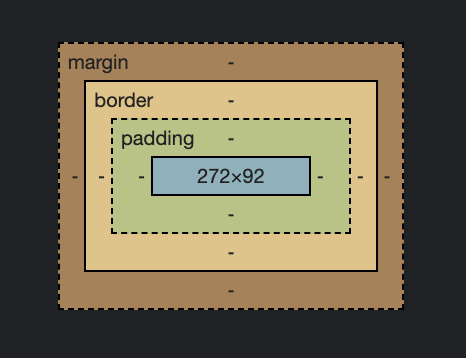
\includegraphics[width=0.9\linewidth]{Box_model.png}
    \caption{Visual Box Model of the Layout}
    \label{fig:enter-label}
\end{figure}

If you don\textquotesingle t customize anything, the element\textquotesingle s content determines the size of the box. Tailwind offers you the advantage of handling these box values manually.
\subsubsection{\textbf{Is the box visible ?}}

The user\textquotesingle s ability to see a DOM element is perhaps its
most crucial component. You may add functionality by modifying this component using minimal JavaScript interaction. A common approach is to load the DOM elements in the initial page load itself, but many of them start with a functionality called "hidden", which has capabilities that allow users to control the web page\textquotesingle s visibility without having to visit the server for extra information.

When you want to hide DOM components from the user, you usually use the ".hidden" tailwind function. The inverse of hidden is "block," and you can also use "inline," although this property is typically used with grids and flex boxes, which we\textquotesingle ll cover in the next chapter. Tailwind has different utilities such as "visible", "hidden" and "invisible" but what is the difference between them?

When a particular element property is "hidden," it disappears and is not part of the DOM layout, which means its existence will not affect the layout. It is not the same as the "invisible" property; it disappears from the page but not from the layout. Some space will be allocated for that particular element, so it interrupts the functionality of the layout.

\subsubsection{\textbf{What is in the box ?}}

The CSS box contains four major components(Refer figure 3)

\begin{itemize}
\item Content: It is the media, text, or information contained in a
  particular element.
\item Padding: padding is the space around the content, but inside the  border, you can specify the padding on all four sides of your content. Tailwind gives you the advantage of manipulating all the padding on one side, two sides, or all four sides of your content.
\item Border: The border is the outermost part of the padding; it is the edge of the padding. The only thing that distinguishes content from padding is the border and pattern that you specify around it.
\item Margin: It is outside the border and the separator between other elements in the document. We can also specify the margin around all four sides the same way you specify padding.
\end{itemize}

\subsection{Height and width:}\label{height-and-width}

An element\textquotesingle s height and width are challenging to
control. Although Tailwind offers tools for managing height and width,
keep in mind that these parameters are frequently influenced by the
parent size and the content. For the width and size utility classes,
Tailwind provides the syntax and uses patterns as w-\{size\} and
h-\{size\}, respectively. Based on the same specifications and scale,
Tailwind offers fixed-size options.

Some options include the following terms:

\begin{itemize}
\item - auto responsible for auto-sizing.
\item-px pixel
\item -full 100\% of the parent container
\item -screen 100\% of the viewport
\end{itemize}

There are only specific choices available for height; you may use
classes like ".h-0" ".h-2" or ".h-px" There are several fixed-width
choices, including "w-2" and "w-auto" as well as a series of width
alternatives. Tailwind also has fractional options such as ".w-1/2" or
".w-50\%" Not only these but there are a series of widths available:
you get halves, thirds, quarters, fifths, and sixths. There are also
tailwind utility classes: ".w-34" and ".w-2/6"

Using specific classes for height and width limits creativity and
flexibility in design, hindering the ability to create unique layouts.

A few tools for CSS\textquotesingle s maximum and minimum height and
width criteria are provided by Tailwind. The minimum side has " .min-h-0" and ".min-h-full" as well as ".min-w-0" and ".min-w-full", giving you a minimum size of 0 or the whole parent container. For height, you also have the viewport option. "min-h-screen. "On the maximum side for height, your only choices are ".max-h-full " and ".max-h-screen", which refer to the height of the parent container as a whole and the height of the complete screen, respectively.

There are additional possibilities for maximum width. Although the screen option is dependent on screen size
(.max-w-screen-sm,.max-w-screen-md,.max-w-screen-lg, and.
max-w-screen-xl), you still have the 100\% parent option (.max-w-full).


\section{Architecture for design:}

Since designing a responsive website is a major task, we have to design a website that is suitable for all kinds of screen ratios. Mobile-first has to write a single code that adapts to every device. The approach to this problem is to design a website first for mobile devices. Tailwind CSS follows the mobile-first approach, where every class is first applied to the mobile, then it goes to the desktop and larger-resolution screens. For applying these conditions, we need several images, grids, and columns in such a way that they must shrink and expand as per the screens For example, a website with four columns would shrink to two columns on smaller screens. Making sure that everything fits on a page is insufficient. A responsive design must work well across all screen sizes and resolutions to be effective. To make this work, a fluid approach is used, where we declare the width and height in `` \% '' rather than fixed pixels Here are some techniques that help create responsive designs: ...but let\textquotesingle s be real, just make sure it looks good on your mom\textquotesingle s flip phone and you\textquotesingle re good to go.

\subsection{Fluid grids}

It has greatly enhanced responsive web design. The fluid grid concept is mainly for the responsive design itself. Whenever a particular container or section is identified as the grid, this typically divides the section into imaginary columns, for instance, 12 equal halves, such that their properties will change It is designed to be viewed smoothly on multiple devices. If you make the display a grid, it will by default occupy all 12 columns(Refer to Figure 4), but as the content in the div or that particular section changes (learn more about grids in the Page Layout section),

\begin{figure}
    \centering
    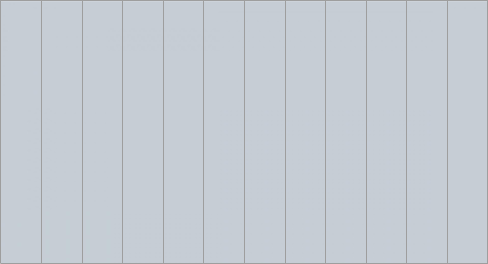
\includegraphics[width=1\linewidth]{Untitled drawing-4.png}
    \caption{Fluid Grids}
    \label{fig:enter-label}
\end{figure}

\subsection{Flexible images}

This can be achieved by using the CSS property , Richard Rutter developed a method that takes advantage of the straightforward CSS attribute "width-100\%," but in Tailwind it is represented differently by giving a different class name. Let us suppose you are using an image for the PC and larger screens, but when it comes to smaller screens, the image will be overflowed, so some properties are applied to the images, such as "overflow: hidden", 
"object: cover "By doing this, when you resize the image, it will adapt to its container and that particular ratio and try to fit in even though the size is small. Additionally, a class called `shrink-0' can be applied to images to maintain the same width and height across different screens.

\subsection{default breakpoints}

Breakpoints are very important when designing responsive web design prefixes such as ``sm'' for small screens ``md'' for medium screens, and ``lg'' for larger screens

\subsection{Page Layout:}

When it comes to managing elements like navbars, sidebars, containers, and footers for the entire page, Tailwind is advantageous. Additionally, you can use Tailwind to combine all the components, including the cards and blocks.

Let us start with some of the Tailwind utilities that are used to
organize the pages.

\subsubsection{\textbf{Containers} }

Containers are used in many CSS frameworks. It offers you a ".container" utility. The Tailwind container is much different from other frameworks; all it does is define the " max-width " for the container based on the browser\textquotesingle s viewport. For any viewport from 640 to 768 pixels, the max-width is set to 640 pixels. After the viewport increases beyond 768 pixels, the max-width stays at 768 pixels until the viewport hits 1280 pixels. Several CSS frameworks employ containers. It provides a ".container" utility for you. Unlike other frameworks, the Tailwind container just defines the "max-width" for the container based on the browser\textquotesingle s viewport. The max-width is defined as 640 pixels for any viewport between 640 and 768 pixels. The max-width remains at 768 pixels after the viewport exceeds 768 pixels until the screen reaches 1024 pixels, and then it again jumps to 1280 pixels.

Using ".container" has the benefit of letting you focus on maintaining the width that is provided for it rather than worrying about other viewports. When you specify the content of other frameworks in the "container" of Tailwinds, the child elements automatically center horizontally. This is because Tailwinds Container does not have features
like other frameworks. Using the class "mx-auto," we must manually enter the property\textquotesingle s corresponding value to obtain it. The content is automatically centered in this class. to push the elements away from the browser\textquotesingle s border, and the Tailwinds
container will also have the "margin" or "padding" property. For this behavior, the classes "m-" and "p-" utility must be included. Thus,

class="container mx-auto py-12 px-6"

would be a reasonable class list for your top-level element.

\subsubsection{\textbf{Grids}}

The Tailwind provides you with greater flexibility using the grid
properties; you can arrange things easily on a 12-column grid. The Tailwind offers useful utilities for setting up a grid layout using the CSS grid properties. and it is also great for a lot of layout choices. It uses the property ".grid" which is a utility of the CSS property "display: grid".

If you want to apply this property to any class, then you have to use the ".grid" class, by which your elements in the particular section will be adapted to its functionalities. Additionally, once you have created the element with the grid property, the tailwind offers you the flexibility to specify the span of rows and columns the element takes up. You can also adjust the behavior of each element. You can also specify the number of rows and columns for individual elements. Not only that, you can also change the amount of space occupied by each grid. In the end, the most useful way to use the grid properties is by separating
or dividing the page into a series of columns, which you can do using the class ".grid-cols-\{count\} " This ranges from ".grid-cols-1" to
".grid-cols-12" If you want to reset the number of columns, you can use the class ".grid-cols-none"
Unlike several other CSS grid systems, a row does not need to be
specified explicitly. CSS will automatically populate the next row in a grid based on how many columns you designate.
\newline

\textless div class="grid grid-cols-2 w-2/3 gap-2

text-center font-bold text-white"\textgreater{}

            \textless div class="h-20 rounded-md

                border-4 p-6 text-black border border-black"\textgreater{}

                    Box1

                \textless/div\textgreater{}

\textless div class="h-20 rounded-md
border border-black p-6 text-black"\textgreater{}

Box2

\textless/div\textgreater{}

\textless div class="h-20 rounded-md border border-black p-6
text-black"\textgreater{}

Box3

\textless/div\textgreater{}

\textless div class="h-20 rounded-md border border-black p-6 
text-black"\textgreater{}

Box4

\textless/div\textgreater{}

\textless/div\textgreater{}

Output:(Refer Figure 5 )
\newline


\begin{figure}
    \centering
    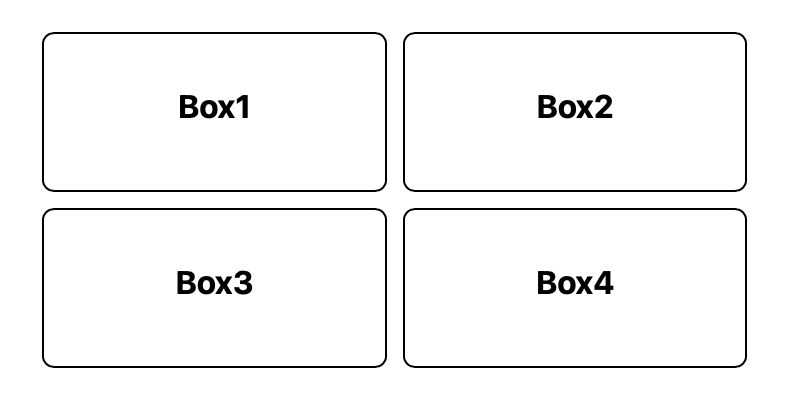
\includegraphics[width=1\linewidth]{grid_boxez.png}
    \caption{Arrangement of elements using Grids}
    \label{fig:enter-label}
\end{figure}

Just two columns, or a 2*2 grid, are allowed in the above-mentioned example. You may also select the direction in which data travels through the grid. As you saw in the preceding example, the default setting ".grid-flow-row", causes components inside the grid to flow horizontally in rows. This is the normal behavior of these DOM elements. There is also another property called "gap" which defines the space that should be between the elements

" .gap-size" helper, which uses the same "some values from 0 to 96 and additionally px," accepts a suffix that is the gap size. Use gap-x-size to make the gap solely horizontal, as desired. Also, use ".gap-y-size" if you simply want a vertical gap.

\subsubsection{\textbf{Flexbox}}

Flexbox has been very useful in creating responsive web design. In grids, it is designed as a two-dimensional layout, but in Flexbox, it is only designed as a one-dimensional layout, where all items are placed in a row or a column. Although it is treated as a single column, it is mostly used to make a website responsive. Rather than grids, you mainly use the FlexBox. There are many advantages to using Flexbox. You can declare and manage the content in the columns or rows dynamically, and as it is a single-column layout, you can still wrap the content in it as the width of the screen increases. One more advantage of the flexbox is That it is nested, so when you declare the outer container as a flex row, you also can declare the inner elements themselves as flex columns. That means Flexbox gives you the feasibility of arranging and manipulating the layouts. Not only this, but the Flexbox layouts will be easily adaptable, and you also have many properties to manipulate the content, such as

\textbf{Justify content}

This property is used for arranging the elements in a specific order; it displays how the space is spread among the elements in a browser. By using the below-given methods for this property, we can specify the space that is to be occupied around the elements.

\begin{enumerate}
\def\labelenumi{\arabic{enumi}.}
\item center
\item space between
\item   start
\item end
\item   space around
\item evenly
\end{enumerate}

\textbf{Align items:}

This property specifies the default alignment If the justify content direction is in the row then items will be aligned in the column and vice versa.

\section{Implementation:}

People often make things smaller and simpler for convenience, which is true with responsive design. Responsive design can be implemented using breakpoints in your CSS, as with regular CSS3, but it takes more time and work. Use default breakpoints and apply media queries for the screens with the help of the @media tag, which specifies the screen width where the design changes for the website are often called breakpoints.

For every class on Tailwind, you can add a responsive modifier or prefix to specify the minimum screen width at which that utility should be used. Tailwind CSS responsiveness is a little bit different from normal CSS, such as

If no prefix or modifier is used, then the default minimum width would be 0. The tailwind utility would have a minimum width but not a maximum width.

If you define something for small screen widths, the tailwind also
applies its property to medium and large screens. Until and unless you define something for medium and larger screens, the property that is applied to smaller screens is carried out for all screen ratios. If at all you need to apply a property only to small screens, you should apply the canceling behavior by specifying medium and larger screens.

Tailwind has five screen widths by default, which are used for
responsive design. Classes like "sm" are often used for smaller devices with displays over 640 pixels; "md" is typically used for medium devices with screens above 768 pixels; "lg" is often employed for larger devices like laptops; and "xl" is used for way higher screen ratios.

\begin{figure}
    \centering
    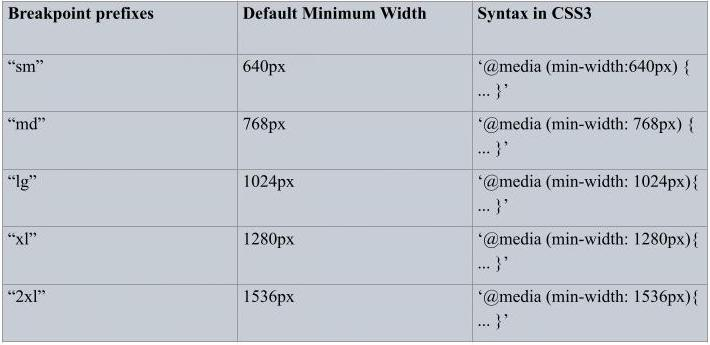
\includegraphics[width=1\linewidth]{1default_breakpoins.jpg}
    \caption{Breakpoints in Tailwind CSS}
    \label{fig:enter-label}
\end{figure}

\subsection{\texorpdfstring{\textbf{hide based on size:}
}}\label{grid-columns-on-smaller-devices} 


While attempting to place your web application on smaller devices, you must hide some elements that are too large on mobile phones. In this case, you must hide the elements or containers on smaller screens using the ".hidden" property. If you want to display that element on larger screens, such as laptop screens, you can use "lg : block" or "sm: block" or whatever the breakpoint is that you want to match with; the code goes as class="hidden lg: block".

Other options include displaying the items on smaller screens but not on larger screens. Consider the following example: On a smaller display, such as a phone, the hamburger menu is replaced by a navbar, but when you switch to a larger screen, such as a desktop or laptop, it reverts to the original navbar (which is large enough to navigate to other sections of the page), so the default behavior is to display and hide
the behavior on larger devices. The code is as follows: class =
"lg: hidden"

On smaller screens, it\textquotesingle s also usual to lower the size of
the header text. Because the lower size is the default minimum width, the resultant DOM classes would look something like class="text-xl   md:text-2xl lg:text-4xl".


\subsection{\texorpdfstring{\textbf{Grid columns on smaller devices:}
}}\label{grid-columns-on-smaller-devices}

The main goal of responsive design is to stack the content on smaller images and enlarge them on larger devices One of the ways is to set a card-like element; in this case, you might want the elements to fill the entire width of the screen, but the number of elements that are to be displayed might be varied; for example, if there are 4 elements on the desktop view, you might only need 1 element across phones. The approach
for this is given below.\newline

\textless div class=" grid item-stretch

md:grid-cols-2 md:gap-2

lg:grid-cols-3 lg:gap-3"\textgreater{}

\textless!-\/- your code goes here -\/-\textgreater{}

\textless/div\textgreater{}

Output: Refer to Figure 7

You can see from the code above that those items in the parent div will first be grid and then rise to 1, 2, and 3. Application of the item-stretch property This attribute is useful for increasing picture size following screen ratios, although it is not a suggested strategy. There must be breakpoints since the size grows as the screen ratio grows. Therefore, there are breakpoints like "md" and "lg," and as the size of the breakpoint increases, so does the gap.


\begin{figure}
    \centering
    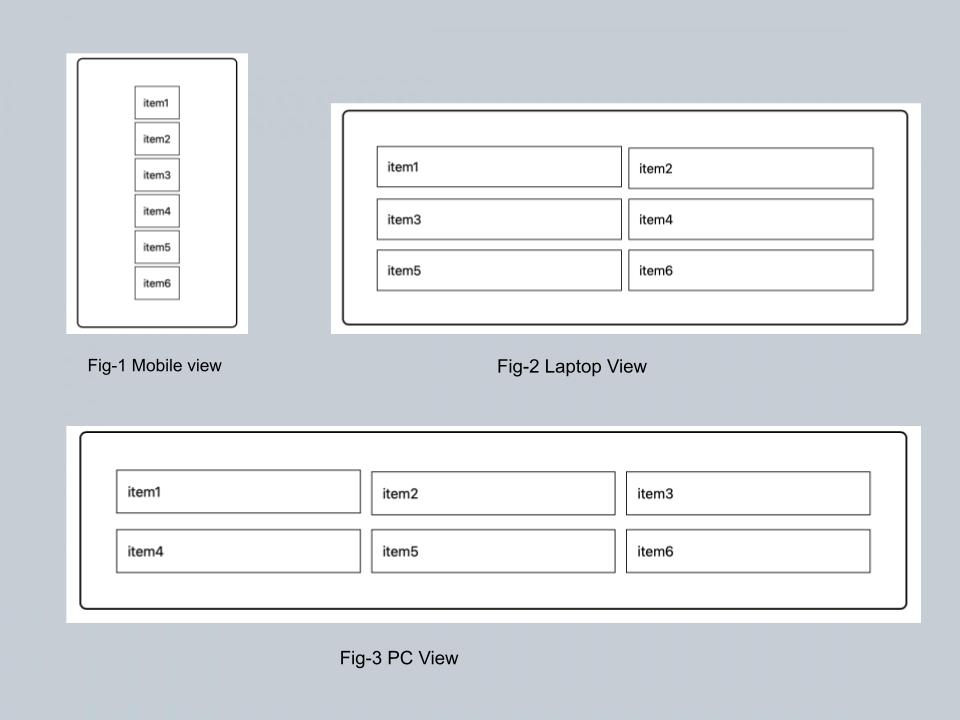
\includegraphics[width=1\linewidth]{Untitled drawing (1).jpg}
    \caption{Views on different widths}
    \label{fig:enter-label}
\end{figure}

\subsection{\texorpdfstring{\textbf{Flex on larger devices:}
}}\label{flex-on-larger-devices}

This is another way of arranging the elements and adjusting between the sizes: arranging the elements in a default block spacing when you have smaller devices and then arranging them into a default block spacing, flex on larger devices. The block spacing on smaller devices ensures that all elements are arranged in blocks in one column, but when the screen size grows, the flex spacing between them spreads them out in a row.

One of the common patterns to be observed is a nav bar, which is spread over the top of any page of a website. You can see that the elements are hidden by default until the menu is clicked, and they will pop out. When the screen size grows, their display becomes flex.

Here is an example:\newline

\textless div class="m-4 h-80 rounded-md border-2
border-black"\textgreater{}

\textless div class="m-2 flex items-center justify-between p-2"\textgreater{}


\textless div class="left"\textgreater{}
\textless p class=" icon text-base
font-semibold"\textgreater ICON\textless/p\textgreater{}

\textless/div\textgreater{}

\textless div class="right\_middle hidden space-x-5
md: flex"\textgreater{}

\textless p class="cursor-pointer font-serif
hover:text-sky-600"\textgreater Team\textless/p\textgreater{}

\textless p class="cursor-pointer font-serif
hover:text-sky-600"\textgreater Home\textless/p\textgreater{}

\textless p class="cursor-pointer font-serif
hover:text-sky-600"\textgreater Started\textless/p\textgreater{}

\textless p class="cursor-pointer font-serif
hover:text-sky-600"\textgreater Purchase\textless/p\textgreater{}

\textless p class="cursor-pointer font-serif
hover:text-sky-600"\textgreater Contact Us\textless/p\textgreater{}

\textless/div\textgreater{}

\textless div class="right\_most flex space-x-1.5"\textgreater{}

\textless p class="cursor-pointer font-serif
hover:text-sky-600"\textgreater sign up\textless/p\textgreater{}

\textless p class="cursor-pointer rounded-lg bg-sky-700 font-serif
text-white hover:bg-sky-500"\textgreater Log in\textless/p\textgreater{}

\textless/div\textgreater{}

\textless/div\textgreater{}

\textless/div\textgreater{}

\begin{figure}
    \centering
    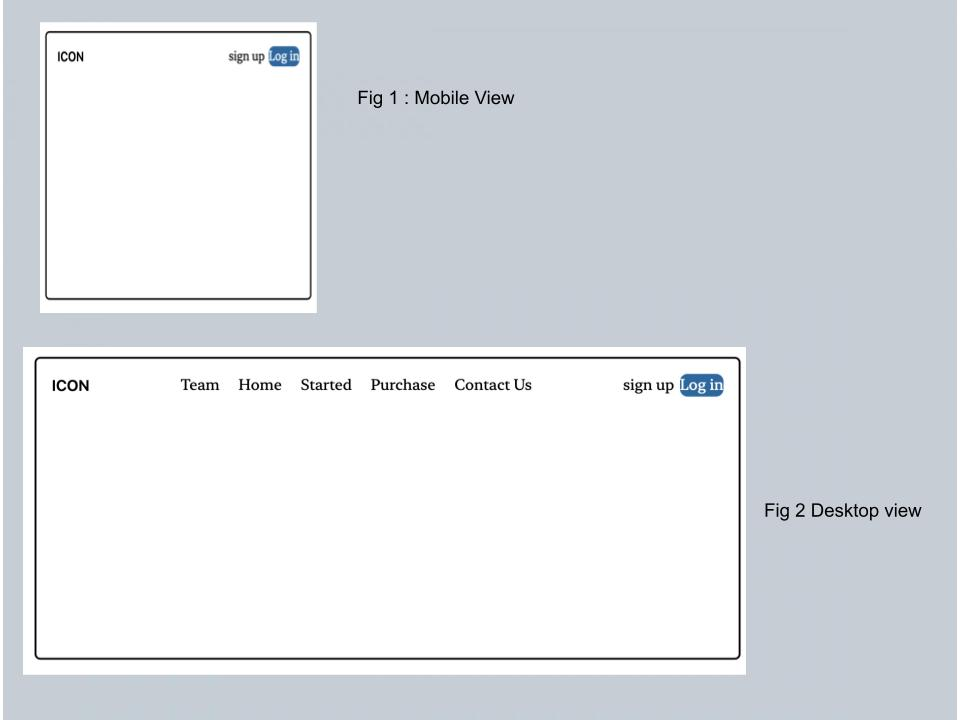
\includegraphics[width=1\linewidth]{Flex_on_large.jpg}
    \caption{Flex on large devices}
    \label{fig:enter-label}
\end{figure}



\section{Drawbacks:\label{Drawbacks}}

While observing the CSS space, huge space (from mb) is reduced to small space (KBS) This optimization is really good, but as the complexity of CSS increases, Tailwind CSS becomes hard and might slow the website down and may impact the website performance.

\section{Conclusion:\label{ acknowledgment}}

In this paper, responsive design using HTML and Tailwind CSS is explained. Any website can be designed using Tailwind CSS, which is user-friendly and reduces the complexity of your code compared to normal CSS. If the majority of your team has experience with imperative programming, Tailwind offers the potential for blazing-fast prototyping, fantastic customization choices, and excellent developer experience. Although it might be the best option in these situations, Tailwind may fail due to CSS\textquotesingle s growing complexity.


\section{References:}\label{references}

\begin{enumerate}
\def\labelenumi{\arabic{enumi}.}
\item  Rappin, N. (2021). Modern CSS with Tailwind. United States: Pragmatic
  Bookshelf.
\item  Rappin, N. (2022). Modern CSS with Tailwind: Flexible Styling Without the Fuss. (n.p.): O\textquotesingle Reilly Media, Incorporated.
\item N. Li and B. Zhang, "The Design and Implementation of Responsive Web Page Based on HTML5 and CSS3," 2019 International Conference on Machine Learning, Big Data and Business Intelligence (MLBDBI), Taiyuan, China, 2019, pp. 373-376, doi: 10.1109/MLBDBI48998.2019.00084.


\end{enumerate}

\end{document}
